\subsection*{Vätgaslampa}
Experimentet ställdes upp enligt beskrivning, varpå tre linjer kunde ses genom spektroskopet. När de uppmätta utgångsvinklarna sätts in i \cref{eq_gitterbrytning}, $k$ sätts till $\pm1$ ($\pm{}$ ty mätningar gjordes för både positiva och negativa vinklar för ökad precision) och $\theta_i=0$ fås \cref{tb_expres_1}; \cref{tb_expres_2} fås då när de värdena sätts in i \cref{eq_gitterbrytning}
\begin{table}[!hb]
	\caption{Experimentellt resultat av mätningar på vätgaslampa. $\theta_j$ är genomsnittet av de två uppmätta vinklarna och den vinkel som används för fortsatta uträkningar.}
	\label{tb_expres_1}
    \begin{center}
    	\renewcommand{\arraystretch}{1.2}
		\begin{tabular}{| c | c | c | c |}
        	\hline
			 & $\theta_{+j}$ & $\theta_{-j}$ & $\theta_{j}$ \\
            \hline
            $\theta_{1}$ & $23.0^\circ$ & $-24.0^\circ$ & $23.5^\circ$ \\
            \hline
            $\theta_{2}$ & $16.75^\circ$ & $-17.75^\circ$ & $17.25^\circ$ \\
            \hline
            $\theta_{3}$ & $14.75^\circ$ & $-15.75^\circ$ & $15.25^\circ$ \\
            \hline
		\end{tabular}
	\end{center}
\end{table}
\begin{table}[!hb]
	\caption{Resulterande experimentell våglängd}
    \label{tb_expres_2}
    \begin{center}
    	\renewcommand{\arraystretch}{1.2}
		\begin{tabular}{| c | c |}
        	\hline
            $\lambda_1$ & $6.6458*10^{-7}$ m \\
            \hline
            $\lambda_2$ & $4.9424*10^{-7}$ m \\
            \hline
            $\lambda_3$ & $4.3839*10^{-7}$ m \\
            \hline
		\end{tabular}
	\end{center}
\end{table}

Enligt \cref{eq_Rydbergs_formel} ger större $m$ mindre $\lambda$ och mindre $\lambda$ i \cref{eq_gitterbrytning} ger mindre $\theta_o$, d.v.s. större $m$ svarar mot mindre $\theta_j$ i enlighet med \cref{tb_expres_1,tb_expres_2}. Det antas att alla språng slutar i det givna grundtillståndet $n=2$ enligt instruktion från labhandledning. 

Från \cref{eq_Rydbergs_formel} fås då tillsammans ovanstående att 
\begin{equation}
	\frac{1}{\lambda_j}=R_H\left(\frac{1}{4}-\frac{1}{(m+j-1)^2}\right)
    \label{eq_lambda_j_1}
\end{equation}
Härifrån definieras $\lambda_j$ för de tre mätvärdena:

\begin{IEEEeqnarray}{r C c}
	\lambda_1 & = & \frac{4}{R_H}\frac{m^2}{(m-2)(m+2)} \nonumber\\
    \lambda_2 & = & \frac{4}{R_H}\frac{(m+1)^2}{(m-1)(m+3)} \IEEEyesnumber\label{eq_lambda(m)_def} \\
    \lambda_3 & = & \frac{4}{R_H}\frac{(m+2)^2}{m(m+4)} \nonumber
\end{IEEEeqnarray}
varpå variablen $F_{ij}(m)$ samt konstanten $\lambda_{ij}$ definieras som 
\begin{equation}
	F_{ij}(m)=\frac{\lambda_i}{\lambda_j}=\lambda_{ij}
    \label{eq_F_def}
\end{equation}
där $F$ kommer från definitionerna i ekvation \ref{eq_lambda(m)_def} medan $\lambda_{ij}$ skapas från de experimentella värdena vilket ger \cref{tb_F_lambda_def}:
\begin{table}[!hb]
	\caption{$F_{ij}(m)$ och $\lambda_{ij}$ tabellerat. Eftersom $F$ för alla $ij$ innehåller den obekanta $4/R_H$ försvinner den vid division vilket låter $m$ räknas ut.} 
    \label{tb_F_lambda_def}
    \begin{center}
    	\renewcommand{\arraystretch}{1.7}
		\begin{tabular}{| c | c c c |}
			\hline
            $ij$ & $F_{ij}(m)$ & = & $\lambda_{ij}$ \\
            \hline
            32 & $\frac{m^2(m-1)(m+3)}{(m+1)^2(m-2)(m+2)}$ & = & 1.3447 \\
            \hline
            31 & $\frac{m^3(m+4)}{(m-2)(m+2)^3}$ & = & 1.5160 \\
            \hline
            21 & $\frac{m(m+1)^2(m+4)}{(m-1)(m+2)^2(m+3)}$ & = & 1.1274 \\
            \hline
		\end{tabular}
	\end{center}
\end{table}

Eftersom $F_{ij}(m)=\lambda_{ij}$ kommer det finnas ett gemensamt $m$ för vilket alla $F_{ij}(m)-\lambda_{ij}=0$, som fås grafiskt till 3:
\begin{figure}[htb]
	\begin{center}
		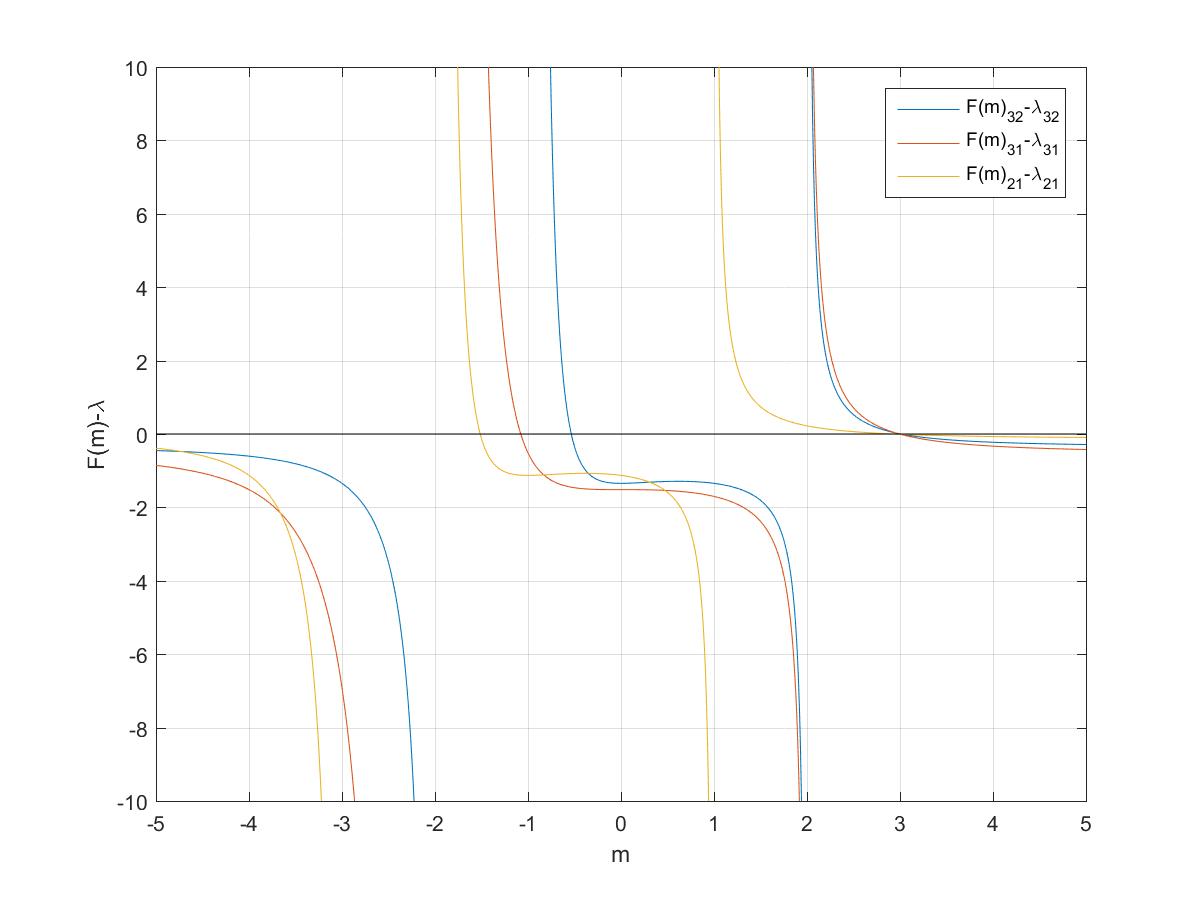
\includegraphics[width=9cm]{Finding_m.png}
        \caption{Enligt figuren passerar alla tre kurvor tillsammans genom 0 nära 3; specifikt 3.011, 2.994 och 2.930 vilket ger medelvärde 2.9783.}
	\end{center}
\end{figure}

När $m=3$ är känt sätts detta tillsammans med  de experimentella våglängderna in i \cref{eq_lambda_j_1} och $R_H$ bryts ut vilket ger \cref{tb_R_H}.
\begin{table}[htb]
	\caption{Numerisk uträkning av $R_H$ från experimentella värden.}
    \label{tb_R_H}
    \begin{center}
    \renewcommand{\arraystretch}{1.3}
		\begin{tabular}{| c c c c c |}
			\hline
            \rule{0pt}{3ex}$R_H(\lambda_1)$ & = & $\left(\lambda_1\frac{5}{36}\right)^{-1}$ & $\approx$ & $1.0834\cdot10^7$ \\
            \hline
            \rule{0pt}{3ex}$R_H(\lambda_2)$ & = & $\left(\lambda_2\frac{12}{64}\right)^{-1}$ & $\approx$ & $1.0791\cdot10^7$ \\
            \hline
            \rule{0pt}{3ex}$R_H(\lambda_3)$ & = & $\left(\lambda_3\frac{21}{100}\right)^{-1}$ & $\approx$ & $1.0862\cdot10^7$ \\
            \hline
            \multicolumn{3}{|l}{Genomsnitt} & $\approx$ & $1.0829\cdot10^{7}$ \\
            \hline
		\end{tabular}
	\end{center}
\end{table}
\Cref{eq_R_Rinf} där $m_e$ är elektronmassan och $M$ är väteatommassan används för att överföra $R_H$ till $R_\infty\approx1.0974\cdot10^7$ för att jämföra med korrekt svar:
\begin{equation}
	\frac{R_H}{\left(1-\frac{m_e}{m_e+M}\right)}\approx1.0835\cdot10^7
    \label{eq_R_Rinf}
\end{equation}

\subsection*{Kvicksilverlampa}
